\documentclass[12pt]{beamer}

\hypersetup{colorlinks=true,linkcolor=red}
\usetheme{default}
\usecolortheme{albatross}

\usepackage[utf8]{inputenc}
\usepackage[russian,english]{babel}
\usepackage[T2A]{fontenc}
\usepackage{hyperref}
\usepackage[final]{listings}
\usepackage{breakurl}
\usepackage{cite}
\usepackage{perpage}

\graphicspath{{img/}}

\def\Url\Breaks{\do\/\do-}
\lstset{
  frame=single,
  breaklines=true,
  basicstyle=\small,
  postbreak=\raisebox{0ex}{\ensuremath{\hookrightarrow\space}},
  numbers=left
}

\MakePerPage{footnote}

\title{Operating Systems}
\subtitle{Hardware Memory and Protection}
\author{Me}
\date{\today}

\begin{document}
  \begin{frame}
    \titlepage
  \end{frame}

  \begin{frame}
\frametitle{Memory Controller (Old, 200x)}
\begin{center}
  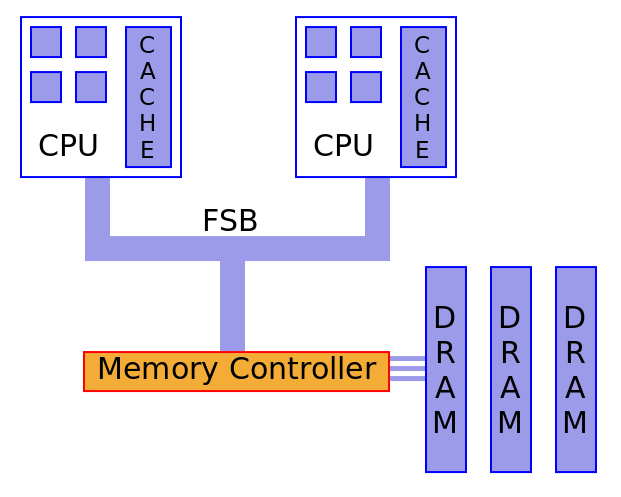
\includegraphics[width=0.8\linewidth]{fsb.png}
\end{center}
\end{frame}

\begin{frame}
\frametitle{Memory Controller (New, 201x)}
\begin{center}
  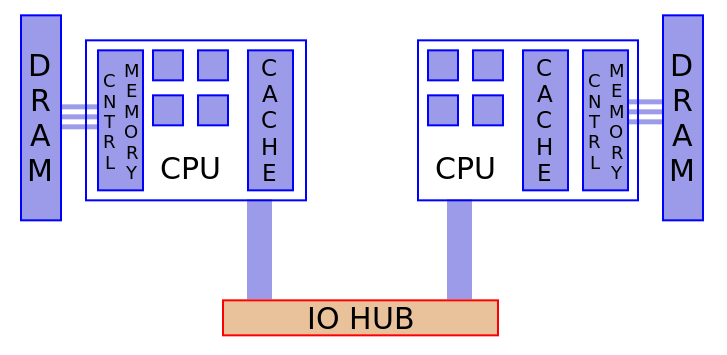
\includegraphics[width=0.8\linewidth]{qpi.png}
\end{center}
\begin{itemize}
  \item CPU видит память через Memory Controller
  \begin{itemize}
    \item подключите к Memory Controller хоть чайник, CPU будет считать его
    памятью.
  \end{itemize}
\end{itemize}
\end{frame}

\begin{frame}
\frametitle{Неоднородность памяти}
\begin{itemize}
  \item Запросы в "память" могут переадресовываться устройствам и иметь побочные
  эффекты:
  \begin{itemize}
    \item например, запись по адресу 0xb8000 приводит к выводу на экран;
    \item обращение по адресу 0xfee00000 переадресуется Local APIC-у;
    \item обращение по адресу 0xfec00000 переадресуется IO APIC-у.
  \end{itemize}
  \item Память по каким-то адресам может отсутсвовать впринципе:
  \begin{itemize}
    \item регионы зарезервированные для устройств отображенных в память и
    неиспользованные;
    \item ISA Hole, участки зарезервированные для PCI и прочих устройств.
  \end{itemize}
\end{itemize}
\end{frame}

\begin{frame}
\frametitle{Карта памяти}
\begin{itemize}
  \item ОС управляет памятью и должна иметь информацию о доступной памяти:
  \begin{itemize}
    \item чтобы настроить алокаторы памяти;
  \end{itemize}
  \item разные системы используют разные интерфейсы для получения карты памяти:
  \begin{itemize}
    \item BIOS, INT 0x15 функция 0xe820;
    \item UEFI, GetMemoryMap();
    \item multiboot (другой загрузчик) может предоставлять карту памяти;
    \item карта памяти может передаваться ОС как аргумент при старте;
    \item \href{https://firmware.intel.com/sites/default/files/resources/A_Tour_Beyond_BIOS_Memory_Map_in\%20UEFI_BIOS.pdf}{A tour beyond BIOS memory map in UEFI BIOS}.
  \end{itemize}
\end{itemize}
\end{frame}

  \begin{frame}
\frametitle{Защита памяти}
\begin{itemize}
  \item От кого/чего нужно защищать память?
  \begin{itemize}
    \item память можно защищать от чтения/записи/исполнения;
    \item память можно защищать от непривилегированного кода;
    \item память одних приложений можно защищать от действий других.
  \end{itemize}
  \item Зачем защищать память?
  \begin{itemize}
    \item защита от непривилегированного кода защищает память ядра ОС от
    действий пользовательских приложений - ошибка в приложении не должна
    приводить к проблемам в ядре;
    \item ошибка в одном приложении не должна вприводить к проблемам в другом.
  \end{itemize}
\end{itemize}
\end{frame}

\begin{frame}
\frametitle{Средства защиты памяти}
\begin{itemize}
  \item Сегментация
  \begin{itemize}
    \item сейчас не особо применяется для защиты памяти;
    \item полезно рассмотреть для домашнего задания.
  \end{itemize}
  \item Paging
  \begin{itemize}
    \item используется для организации трансляции адресов - дает уровень
    косвенности при работе с памятью;
    \item позволяет защищать память на уровне отдельно взятых "страниц";
    \item является основным инструментом для защиты памяти сейчас;
    \item на x86 используется "совместно" с сегментацией.
  \end{itemize}
  \item Другие архитектурно зависимые средства...
\end{itemize}
\end{frame}

\begin{frame}
\frametitle{Сегментация на примере x86}
\framesubtitle{Сегментные регистры}
\begin{itemize}
  \item В x86 при любом обращении к памяти явно или неявно используется один из
  сегментых регистров:
  \begin{itemize}
    \item DS, ES, CS, SS, FS, GS.
  \end{itemize}
  \item Если регистр не указан явно, то регистр выбирается в зависимости от
  операции:
  \begin{itemize}
    \item для обычных чтения и записи данных используются DS или ES;
    \item для операций работы со стеком (push, pop и др.) используется SS;
    \item для чтения следующей инструкции из памяти используется CS;
    \item FS и GS... Ну это отдельная история...
  \end{itemize}
\end{itemize}
\end{frame}

\begin{frame}
\frametitle{Сегментация на примере x86}
\framesubtitle{Селектор сегмента}
\begin{center}
  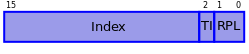
\includegraphics[width=0.4\linewidth]{rpl.png}
  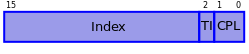
\includegraphics[width=0.4\linewidth]{cpl.png}
\end{center}
\begin{itemize}
  \item Сегментный регистр хранит 16-битное значение - селектор сегмента:
  \begin{itemize}
    \item RPL - Requested Priviledge Level (DS, ES, FS, GS, SS);
    \item CPL - Current Priviledge Level (CS);
    \item TI - Table Indicator (0 - GDT, 1 - LDT);
    \item Index - индекс записи в таблице (GDT или LDT, в зависимости от TI).
  \end{itemize}
\end{itemize}
\end{frame}

\begin{frame}
\frametitle{Сегментация на примере x86}
\framesubtitle{Уровни привилегий 1/2}
\begin{center}
  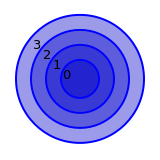
\includegraphics[width=0.3\linewidth]{priv.png}
\end{center}
\begin{itemize}
  \item В x86 есть 4 уровня привелегий (aka ring0 - ring3):
  \begin{itemize}
    \item 0-ой - наивысший уровень привилегий, на этом уровне можно выполнять
    любые инструкции и обращаться к любой памяти;
    \item 3-ий - низший уровень, на этом уровне некоторые инструкции не
    доступны, и доступ к памяти может быть ограничен.
  \end{itemize}
\end{itemize}
\end{frame}

\begin{frame}
\frametitle{Сегментация на примере x86}
\framesubtitle{Уровни привилегий 2/2}
\begin{itemize}
  \item На уровне 0, \emph{обычно}, работает ядро ОС:
  \begin{itemize}
    \item ядро ОС должно иметь полный контроль над системой;
    \item два младших бита в CS у ядра ОС, обычно, равны 0;
  \end{itemize}
  \item на уровне 3, \emph{обычно}, работают пользовательские приложения:
  \begin{itemize}
    \item редакторы текста, браузеры, компиляторы и прочее;
    \item в том числе и QEMU (если оставить в стороне KVM);
    \item два младших бита в CS у приложений, обычно, равны 3;
  \end{itemize}
  \item уровни 1 и 2 используются редко и в очень специфичных приложениях.
\end{itemize}
\end{frame}

\begin{frame}
\frametitle{Сегментация на примере x86}
\framesubtitle{Сегментные дескрипторы}
\begin{itemize}
  \item Index - индекс записи в GDT и LDT:
  \begin{itemize}
    \item в обоих таблица записи имеют одинаковый формат и значение, т. ч. для
    нас между ними нет разницы.
  \end{itemize}
  \item Смысл записей в GDT/LDT немного меняется в зависимости от режима работы
  процессора
  \begin{itemize}
    \item в Real Mode нет защиты памяти;
    \item в данном контексте нас интересуют только Protected Mode и Long Mode.
  \end{itemize}
  \item Дескрипторы в GDT/LDT делятся на системные и все остальные
  \begin{itemize}
    \item системные дескрипторы используются для специфичных нужд x86;
    \item в данном контексте нас не интересуют системные дескрипторы.
  \end{itemize}
\end{itemize}
\end{frame}

\begin{frame}
\frametitle{Сегментация на примере x86}
\framesubtitle{Сегментные дескрипторы в Protected Mode 1/2}
\begin{center}
  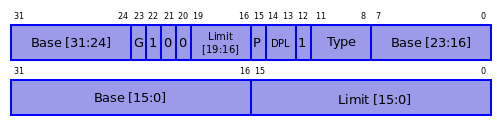
\includegraphics[width=0.6\linewidth]{gdt32.png}
\end{center}
\begin{itemize}
  \item Protected Mode дескриптор содержит
  \begin{itemize}
    \item Base и Limit - описывают границы региона физической памяти;
    \item DPL - Descriptor Priviledge Level;
    \item TYPE - тип сегмента (сегмент кода/данных, разершено ли чтение/запись);
    \item P - бит присутсивия (должен быть 1 для валидных сегментов);
    \item G - бит гранулярности (1 - Limit в 4Kb блоках, 0 - Limit в байтах).
  \end{itemize}
\end{itemize}
\end{frame}

\begin{frame}
\frametitle{Сегментация на примере x86}
\framesubtitle{Сегментные дескрипторы в Protected Mode 2/2}
\begin{center}
  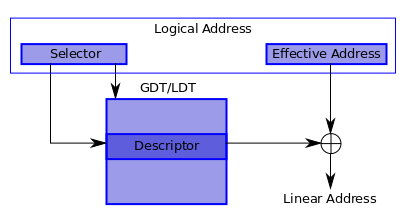
\includegraphics[width=0.55\linewidth]{segtr.png}
\end{center}
\begin{itemize}
  \item Указатель в программе (aka логический адрес) состоит из двух частей:
  \begin{itemize}
    \item сегментного регистра (CS, DS, ES, SS, FS, GS);
    \item смещения (aka эффективный адрес).
  \end{itemize}
  \item Логический адрес пробразуется в линейный адрес
  \begin{itemize}
    \item при преобразовании проверяется, что эффективный адрес не больше Limit.
  \end{itemize}
\end{itemize}
\end{frame}

\begin{frame}
\frametitle{Сегментация на примере x86}
\framesubtitle{Сегментные дескрипторы в Long Mode}
\begin{center}
  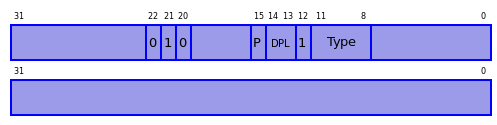
\includegraphics[width=0.6\linewidth]{gdt64.png}
\end{center}
\begin{itemize}
  \item Long Mode дескриптор содержит почти то же самое что и в Protected Mode
  \begin{itemize}
    \item Base и Limit потеряли свой смысл, т. е. трансляция логического адреса
    в линейный не выполняется и границы сегмента не проверяются;
    \item кроме того нельзя ограничить память, описываемую сегментным
    дескриптором, т. е. сегментация как самостоятельный способ защиты теряет
    свой смысл;
    \item кроме регистров FS и GS.
  \end{itemize}
\end{itemize}
\end{frame}

\begin{frame}
\frametitle{Сегментация на примере x86}
\framesubtitle{Проверка уровня привилегий при доступе к данным}
\begin{itemize}
  \item При загрузке селектора в сегментный регистр (DS, ES, FS, GS) CPU
  выполняет проверку уровня привелегий:
  \begin{itemize}
    \item в проверке участвуют текущий CPL, RPL в значении селектора и DPL в
    дескрипторе сегмента, соответствующего селектору;
    \item DPL должен быть численно больше или равен и CPL и RPL, в противном
    случае генерируется исключение;
    \item ОС задает селекторы приложения, и приложение очень ограничено в их
    изменении.
  \end{itemize}
  \item Для сегмента стека SS проверка немного другая:
  \begin{itemize}
    \item RPL и CPL должны совпадать с DPL;
    \item на практике для данных и стека часто используют один дескриптор.
  \end{itemize}
\end{itemize}
\end{frame}

\begin{frame}
\frametitle{Страничная организация памяти}
\begin{itemize}
  \item Страничная организация памяти (Paging) - постраничная трансляция адресов
  \begin{itemize}
    \item физическое адресное пространство разбивается на страницы;
    \item логическое/линейное адресное пространство так же разбивается на
    страницы;
    \item ОС настраивает отображение страниц логического/линейного адресного
    простанства на страницы физического;
    \item CPU транслирует логический/линейный адрес в физический пользуясь
    отображением при обращених в память;
    \item в отображении так же можно задать уровень привилегий доступа, права
    на запись и исполнение.
  \end{itemize}
\end{itemize}
\end{frame}

\begin{frame}
\frametitle{Paging на примере x86}
\framesubtitle{Таблица страниц}
\begin{center}
  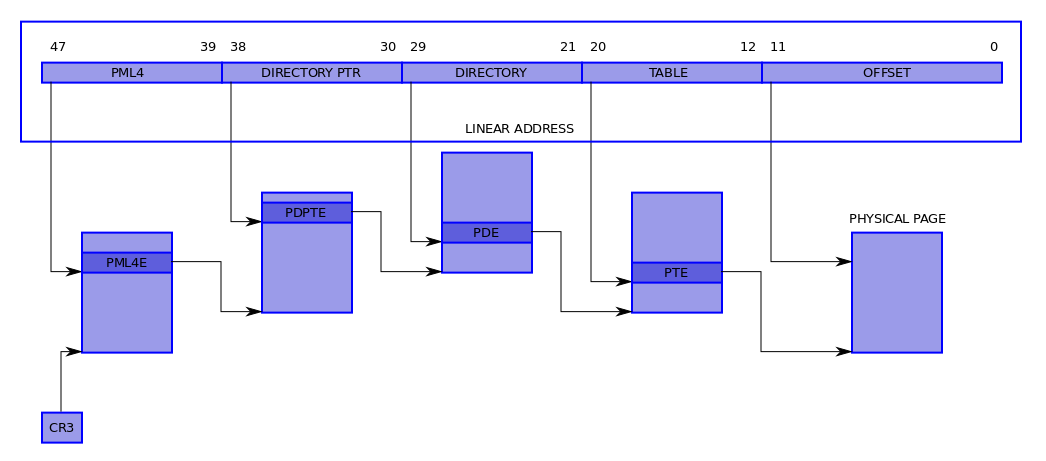
\includegraphics[width=0.55\linewidth]{paging.png}
\end{center}
\begin{itemize}
  \item Для трансляции линейного адреса в физический используется иеархическая
  структура:
  \begin{itemize}
    \item узел дерева - 4KB таблица, 512 записей в каждой;
    \item физический адрес корня хранится в специальном регистре \emph{cr3};
    \item запись в таблице содержит физический адрес таблицы следующего уровня;
    \item смещение в таблице берется из линейного адреса.
  \end{itemize}
\end{itemize}
\end{frame}

\begin{frame}
\frametitle{Paging на примере x86}
\framesubtitle{Замечания о таблице страниц}
\begin{itemize}
  \item Различные линейные адреса легко могут быть отображены на один
  физический:
  \begin{itemize}
     \item например, мы можем создать одну страничку заполненную нулями и
     отобразить все странички, которые должны быть занулены на нее.
  \end{itemize}
  \item \emph{Обычно} у каждого пользовательского приложения своя таблица
  страниц:
  \begin{itemize}
    \item таким образом память одних приложений может быть изолирована от памяти
    других приложений;
    \item при этом разные таблицы страниц могут также ссылаться на одну и ту же
    физическую память.
  \end{itemize}
\end{itemize}
\end{frame}

\begin{frame}
\frametitle{Paging на примере x86}
\framesubtitle{PML4 Entry}
\begin{center}
  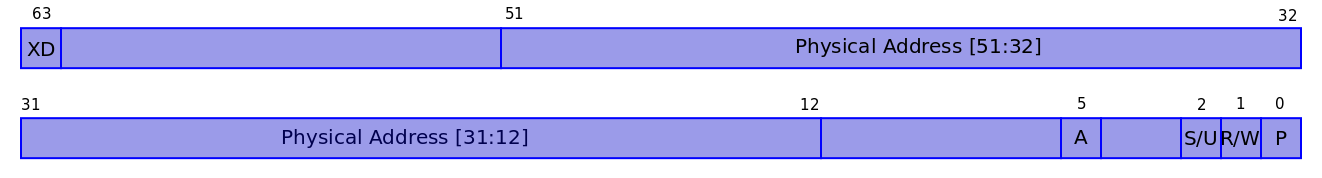
\includegraphics[width=0.9\linewidth]{pml4e.png}
\end{center}
\begin{itemize}
  \item P (Present) - если 0, то запись не валидна, иначе запись валидна;
  \item R/W - если 0, то запись запрещена, иначе разрешена;
  \item S/U - если 0, то доступ разрешен только для привилегированного кода;
  \item XD - если 1, то исполнение кода запрещено (специальная фича, требует
  включения);
  \item A - автоматически выставляется в 1, если запись была использована для
  CPU для трансляции адресов;
  \item Physical Address - физический адрес таблицы следующего уровня;
\end{itemize}
\end{frame}

\begin{frame}
\frametitle{Paging на примере x86}
\framesubtitle{PDPT и PDT Entries}
\begin{center}
  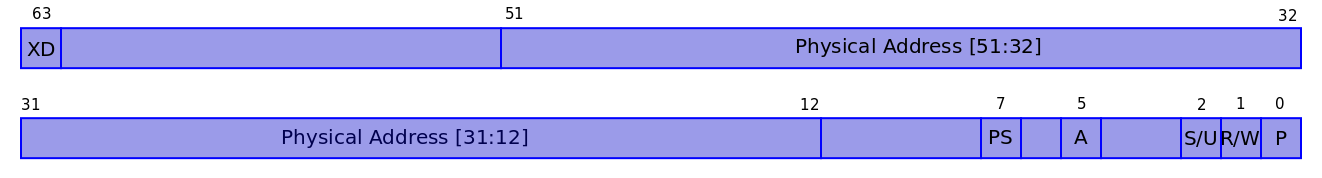
\includegraphics[width=0.9\linewidth]{pdpte.png}
\end{center}
\begin{itemize}
  \item PS (Page Size) - если 1, то Physical Address хранит адрес 1GB или 2MB
  страницы (в PDPT 1GB, в PDT 2MB) физической памяти, в противном случае адрес
  таблицы следующего уровня;
  \item т. е. не все страницы в отображении всегда одного размера.
\end{itemize}
\end{frame}

\begin{frame}
\frametitle{Paging на примере x86}
\framesubtitle{Замечания о таблице страниц}
\begin{itemize}
  \item Одна запись в PML4 описывает 512 GB линейного адресного пространства:
  \begin{itemize}
    \item все запреты в PML4E распространяются на весь 512 GB регион независимо
    от того, что написано в записях нижних уровней;
  \end{itemize}
  \item одна запись в PDPT описывает 1 GB линейного адресного пространства;
  \item одна запись в PDT описывает 2 MB линейного адресного пространства;
  \item одна запись в PD описывает 4 KB линейного адресного пространства:
  \begin{itemize}
    \item 4 KB - наименьшая возможная гранулярность в x86.
  \end{itemize}
\end{itemize}
\end{frame}

\begin{frame}
\frametitle{Канонический адрес}
\begin{itemize}
  \item Из линейного адреса в x86 используется всего 48 бит, но указатель 64
  битный
  \begin{itemize}
    \item биты 63-48 должны быть равны биту 47;
    \item т. е. если бит 47 установлен, то и биты 64-48 тоже должны быть равны
    1, в противном случае они должны быть равны 0.
  \end{itemize}
  \item На адреса в x86 можно смотреть как на числа со знаком:
  \begin{itemize}
    \item есть два региона допустимых адресов $\left[0, 2^{47}\right)$ и
    $\left(-2^{47}, -1\right]$;
    \item отрицательные 64-битное число $x$ представляется с использованием
    дополнения до 2 как беззнаковое число $2^{64} - x$.
  \end{itemize}
\end{itemize}
\end{frame}

  \begin{frame}
\frametitle{Page Fault}
\begin{itemize}
  \item Ошибки трансляции адресов:
  \begin{itemize}
    \item при трансляции адресов бит P может быть сброшен в одной из записей;
    \item может произойти нарушение привелегий - непривилегированный код
    пытается читать/писать память только для привилегированного кода;
    \item нарушение прав доступа, запись/исполнение в/из памяти доступной только
    на чтение.
  \end{itemize}
  \item При подобных ошибках полезно знать:
  \begin{itemize}
    \item адрес, к которому происходило обращение;
    \item какое обращение к памяти происходило (чтение/запись/исполнение) или
    какого рода ошибка произошла.
  \end{itemize}
\end{itemize}
\end{frame}

\begin{frame}
\frametitle{Page Fault в x86}
\framesubtitle{Код ошибки при Page Fault}
\begin{center}
  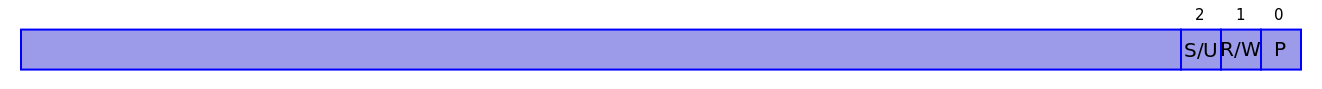
\includegraphics[width=0.9\linewidth]{pferr.png}
\end{center}
\begin{itemize}
  \item P - 0, если Page Fault произошел из-за сброшенного бита P в одной из
  записей;
  \item R/W - 0, если Page Fault произошел при чтении, в проивном случае Page
  Fault произошел при запси;
  \item S/U - 0, если Page Fault произошел в привилегированном коде, в противном
  случае Page Fault произошел в непривилегированном коде.
\end{itemize}
\end{frame}

\begin{frame}
\frametitle{Page Fault в x86}
\framesubtitle{Адрес доступа и адрес возврата}
\begin{itemize}
  \item Адрес, обращение к которому вызвало Page Fault, сохраняется в
  специальный регистр \emph{cr2}.
  \item Адрес возврата, который сохраняется на стек перед вызовом обработчика
  исключения, содержит адрес инструкции, которая привела к Page Fault
  \begin{itemize}
    \item т. е. по возращению из обработчика исключения инструкция будет
    выполнена заново;
    \item т. е. обработчик исключения может поправить отображение после чего
    инструкция будет выполнена заново.
  \end{itemize}
\end{itemize}
\end{frame}

\begin{frame}
\frametitle{Page Fault в x86}
\framesubtitle{Пример: оптимизация memcpy больших регионов 1/3}
\begin{center}
  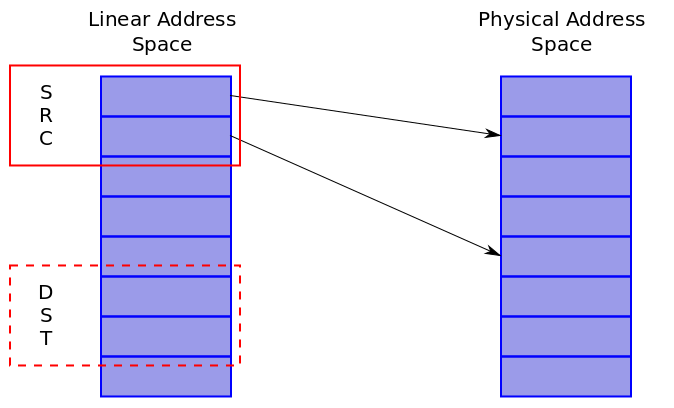
\includegraphics[width=0.6\linewidth]{memcpy0.png}
\end{center}
\begin{itemize}
  \item Хотим скопировать SRC в DST (для простоты регионы выровнены на 4 KB)
  \begin{itemize}
    \item SRC каким-то образом отображено на физическую память;
    \item отображение DST нас не особо интересует.
  \end{itemize}
\end{itemize}
\end{frame}

\begin{frame}
\frametitle{Page Fault в x86}
\framesubtitle{Пример: оптимизация memcpy больших регионов 2/3}
\begin{center}
  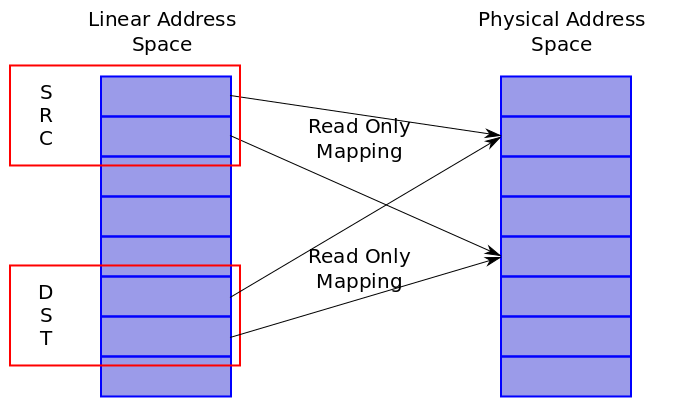
\includegraphics[width=0.6\linewidth]{memcpy1.png}
\end{center}
\begin{itemize}
  \item Вмеcто копирования памяти отображаем DST на те же страницы, что и SRC
  \begin{itemize}
    \item оба оторбажения должны быть Read Only, чтобы модификация приводила к
    Page Fault.
  \end{itemize}
\end{itemize}
\end{frame}

\begin{frame}
\frametitle{Page Fault в x86}
\framesubtitle{Пример: оптимизация memcpy больших регионов 3/3}
\begin{center}
  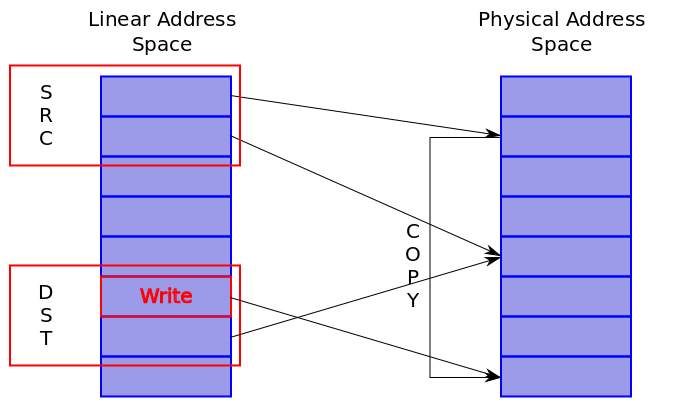
\includegraphics[width=0.6\linewidth]{memcpy2.png}
\end{center}
\begin{itemize}
  \item Попытка записи в SRC или DST приводит к Page Fault:
  \begin{itemize}
    \item в обработчике Page Fault мы можем на самом деле скопировать страницу
    памяти;
    \item таким образом мы реально копируем только те страницы, которые будут
    изменяться и только тогда, когда они будут изменяться.
  \end{itemize}
\end{itemize}
\end{frame}



  \begin{frame}
  \begin{center}
  \Huge Q\&A
  \end{center}
  \end{frame}
\end{document}
